\documentclass[conference]{IEEEtran}
\usepackage[T1]{fontenc}
\usepackage{amsmath,amssymb}
\usepackage{booktabs}
\usepackage{url}
\usepackage[hidelinks]{hyperref}
\usepackage{xcolor}
\usepackage{tikz}
\usetikzlibrary{positioning,arrows.meta}
\newcommand{\pres}{\textsf{preserved}}
\newcommand{\viol}{\textsf{violated}}
\newcommand{\unres}{\textsf{unresolved}}
\newcommand{\code}[1]{\texttt{\small #1}}

\begin{document}

\title{Did the Agent Stay Within Its Authority?\\ Portable Evidence and a Mutation-Hardened Conformance Suite}

\author{\IEEEauthorblockN{Staford Titus Selvaraj}
\IEEEauthorblockA{Independent Researcher\\
stafordtituss@gmail.com\\
ORCID 0009-0004-8227-7595}}

\maketitle

\begin{abstract}
Agentic systems act for people through chains of sub-agents, tools and adapters. Identity establishes who acted and authorization establishes what a token allowed, but neither lets a third party check whether what was actually executed stayed within what a person authorized. We present the Agentic Mandate Evidence Protocol (AMEP), an open specification for portable, signed evidence of each link in that chain, from a person's mandate through delegations and invocations to an independently observed executed effect, and a deterministic, three-valued evaluation over it that returns \pres{}, \viol{} or \unres{}. Missing or unverifiable evidence yields \unres{}, never permission. We treat the specification as a software artefact whose verifiers must be tested, and report three engineering results. First, two independently written verifiers (Python and JavaScript) agree on all 111 vectors of the conformance suite and on a 20-vector delegation suite built for a W3C agent-identity community group. Second, mutation analysis of the reference evaluator showed that the original 95-vector suite detected only 53 of 70 seeded faults; the surviving mutants pointed to untested rules and inclusive bounds, and 16 vectors derived from them raised detection to 69 of 70, with the remaining mutant equivalent under the schema. Third, evaluation costs under 1\,ms per packet and grows linearly with delegation depth. We also report an MCP prototype in which tool servers return signed receipts of the effects they executed.
\end{abstract}

\begin{IEEEkeywords}
agentic AI, delegation, authorization, audit evidence, conformance testing, mutation analysis, Model Context Protocol
\end{IEEEkeywords}

\section{Introduction}

An agent acting for a person rarely acts directly. A user asks a host agent; the host spawns sub-agents; sub-agents call tools through adapters; adapters turn calls into effects on files, SaaS records, payment systems or other people's inboxes. At every hop, what is done can drift from what was asked. An approval for one command can be replayed for another. A sub-agent can receive broader scope than its parent held. Untrusted content can steer a mutation. An adapter can map a declared call to a different effect. A revoked grant upstream can leave a live child downstream. And an enforcement point can say ``deny'' on a host that runs the action anyway.

When something goes wrong, the people who must answer for it (an operator, an auditor, a regulator, the affected user) need to establish what happened and whether it was authorized. Today they reconstruct this from logs written by the systems under scrutiny, in formats that differ per vendor, with no way to tell ``the agent did this'' from ``the agent said it did this''. Existing standards address adjacent questions. OAuth 2.0 Token Exchange~\cite{rfc8693} issues delegated tokens; OpenID AuthZEN~\cite{authzen} transports access decisions; SCITT~\cite{scitt} makes records tamper-evident; capability tokens such as Macaroons~\cite{macaroons}, Biscuit~\cite{biscuit} and UCAN~\cite{ucan} make attenuation structural. None states, in a form a third party can check offline, whether an executed effect stayed within the authority that was delegated, or what to conclude when the evidence needed to decide is missing.

The Agentic Mandate Evidence Protocol (AMEP) fills that gap. It is published as an IETF Internet-Draft~\cite{amepid} with open-source verifiers~\cite{amep}. This paper takes a software-engineering view of it: a protocol whose value lies in independent parties reaching the same verdict on the same evidence is only as good as the tests that pin that verdict down. Our contributions are:
\begin{itemize}
\item an evidence model that separates identity, authority, declared action, executed effect and approval into objects signed by keys holding role-restricted permissions (Section~\ref{sec:model});
\item a claim algebra and eleven invariants with a deterministic, three-valued evaluation in which missing evidence is never permission (Sections~\ref{sec:algebra}--\ref{sec:eval});
\item a conformance suite, two independently written verifiers that agree on it, and a mutation analysis that measures how well the suite pins down evaluator behaviour and guided 16 additional vectors (Sections~\ref{sec:conf}--\ref{sec:results});
\item two integrations: signed effect receipts for Model Context Protocol (MCP) tool calls, and delegation-continuity vectors for an agent-identity registry (Section~\ref{sec:integrations}).
\end{itemize}

\section{Problem and Threat Model}

A principal $H$ authorizes an agent $A$, which may delegate to agents $B, C, \dots$, which invoke tools $T$. A relying party (a receiving tool, an auditor or a regulator) wants to know, for each executed effect: whose authority it was exercised under; whether that authority narrowed or widened along the chain; whether the executed effect matched what was declared; whether any approval covered exactly that effect; and whether any link had been revoked at the time.

AMEP assumes that every language model in the chain may be adversarial, so nothing a model says about itself counts as evidence. Hosts, adapters and observers are trusted only for the statements their keys are entitled to sign. We assume Ed25519~\cite{rfc8032} is unforgeable and that verifiers obtain authentic key sets with role assignments. AMEP does not detect prompt injection, issue identities or define a policy language; it records the findings of such systems and evaluates the evidence they leave. Three principles follow. \emph{Declared $\neq$ executed:} what an agent declares and what a system executed are recorded separately and compared. \emph{Fail-safe evidence:} missing, unsigned or unverifiable evidence yields \unres{}, never \pres{}. \emph{Independent observation:} effects that write shared state, send data externally, destroy data or move money need an observer other than the actor.

\section{Evidence Model}\label{sec:model}

A \emph{packet} is a set of signed JSON objects submitted together for evaluation. Each object is signed with Ed25519 over its RFC~8785 (JCS)~\cite{rfc8785} canonical form, excluding the proof. Every key carries roles, and a verifier treats an object as unsigned unless its key holds a role permitted for the object's kind (Table~\ref{tab:objects}). Without roles, a compromised host key could mint its own mandate or approve its own action and the evidence would still verify.

\begin{table}[t]
\caption{Evidence objects and the signer roles permitted for each}\label{tab:objects}
\centering\footnotesize
\begin{tabular}{@{}p{1.55cm}p{1.35cm}p{5.1cm}@{}}
\toprule
Object & Role & States \\
\midrule
Mandate & issuer & root claim set granted for a principal \\
Delegation & issuer, host & claim set for a delegate; names its parent \\
Intent & issuer, host & narrower per-request claim set \\
Interpretation & host & adapter mapping of a tool call, versioned \\
Invocation & host & declared action, resource, effect class \\
Effect receipt & observer & what was executed; assurance L0--L3 \\
Approval & approver & human approval bound to one effect digest \\
Revocation, status & issuer & signed revocation or status as of a time \\
Decision & host & allow/deny/hold/quarantine with its phase \\
\bottomrule
\end{tabular}
\end{table}

\begin{figure}[t]
\centering
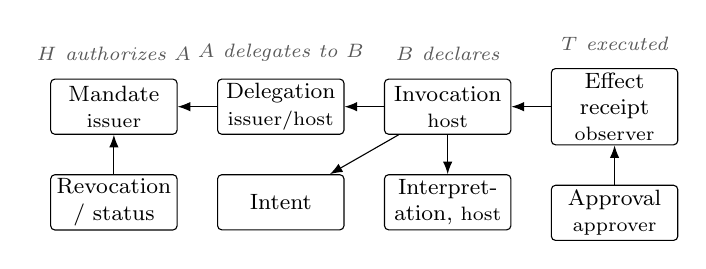
\begin{tikzpicture}[font=\footnotesize, node distance=4mm and 5mm,
  obj/.style={draw, rounded corners=1.5pt, align=center, minimum height=7mm, inner sep=1.5pt, text width=15mm},
  who/.style={font=\scriptsize\itshape, text=black!65},
  arr/.style={-{Latex[length=1.6mm]}}]
\node[obj] (m) {Mandate\\{\scriptsize issuer}};
\node[obj, right=of m] (d) {Delegation\\{\scriptsize issuer/host}};
\node[obj, right=of d] (i) {Invocation\\{\scriptsize host}};
\node[obj, right=of i] (e) {Effect receipt\\{\scriptsize observer}};
\node[obj, below=5mm of m] (r) {Revocation\\/ status};
\node[obj, below=5mm of d] (n) {Intent};
\node[obj, below=5mm of i] (a) {Interpret-\\ation, {\scriptsize host}};
\node[obj, below=5mm of e] (p) {Approval\\{\scriptsize approver}};
\draw[arr] (d) -- (m);
\draw[arr] (i) -- (d);
\draw[arr] (e) -- (i);
\draw[arr] (r) -- (m);
\draw[arr] (i) -- (n);
\draw[arr] (i) -- (a);
\draw[arr] (p) -- (e);
\node[who, above=1mm of m] {$H$ authorizes $A$};
\node[who, above=1mm of d] {$A$ delegates to $B$};
\node[who, above=1mm of i] {$B$ declares};
\node[who, above=1mm of e] {$T$ executed};
\end{tikzpicture}
\caption{Evidence for one executed effect. Arrows point from an object to the object it references (parent, authority, invocation, intent, adapter, revocation target, approved effect digest); each object is signed by a key holding the role shown. The verifier checks the chain, compares the declared invocation with the observed receipt, and checks that any approval is bound to the digest of exactly that effect.}\label{fig:chain}
\end{figure}

Figure~\ref{fig:chain} shows how the objects reference each other. Two choices are central. First, the executed effect is \emph{observed}, not claimed: the receipt is signed by the system where the action took effect, or by a proxy or host hook, and carries an assurance level from L0 (self-reported) to L3 (the receiving system). Second, decisions carry a \emph{phase} (pre-execution, post-execution or simulation), so detection after the fact is never presented as enforcement.

\section{Claim Algebra}\label{sec:algebra}

Authority is a claim set $C$: action and resource patterns, permitted data flows (class$\to$recipient), an effect-class ceiling from the chain \code{read} $<$ \code{write\_local} $<$ \code{write\_shared} $<$ \code{external\_send} $<$ \code{destructive} $<$ \code{financial}, a validity window, an optional purpose, deny lists, an optional risk budget and a delegation depth.

\emph{Order.} $C_1 \sqsubseteq C_2$ (the child is equal to or narrower than the parent) holds when every child pattern is subsumed by a parent pattern; the child's data flows are a subset; its ceiling, expiry and budget are no greater and its not-before no earlier; its purpose is unchanged; its deny lists cover every parent deny; and the depth rule holds (a parent of depth 0 may not be delegated, and otherwise the child's depth is strictly smaller).

\emph{Meet.} $C_1 \sqcap C_2$ is computed component-wise, with the union of deny lists so that no hop and no intent can lift a deny. The effective claims of an invocation are the meet of every claim set on its chain, met again with its intent when one is cited.

\emph{Satisfaction.} An executed effect $x \models C$ when its action and resource match an allowed pattern and no deny, its effect class is within the ceiling, every released data flow is permitted, and its time lies in the (inclusive) window.

These relations use only pattern subsumption, set inclusion and comparison, so they are decidable and cheap, and adding a hop can never widen effective claims. Capability tokens enforce the same rule structurally: a widened Macaroon simply fails to verify. AMEP instead records each delegation as a separately signed claim set and checks $\sqsubseteq$ afterwards, so a widening is \emph{reported} as a violation naming the responsible hop. The two compose: tokens can carry mandates and delegations, and AMEP profiles map their facts onto claims.

\section{Invariants and Evaluation}\label{sec:eval}

\begin{table}[t]
\caption{Invariants and the outcome when each is broken (V: \viol{}, U: \unres{})}\label{tab:inv}
\centering\footnotesize
\begin{tabular}{@{}p{0.55cm}p{6.1cm}p{0.9cm}@{}}
\toprule
ID & Statement (abridged) & Broken \\
\midrule
I1 & Every delegation $\sqsubseteq$ its parent & V \\
I2 & Executed matches declared, satisfies effective claims, within budget unless approved & V \\
I3 & Adapter mapping approved and pinned & U \\
I4 & Untrusted content did not steer a mutation unconfirmed & V/U \\
I5 & Every released data flow permitted & V \\
I6 & No link revoked at or before the invocation & V \\
I7 & Evidence present, well formed, role-signed, fresh & U \\
I8 & Approval matches executed body, in window, used once & V \\
I9 & No action targets guardrails, keys or evidence store & V \\
I10 & High-impact effects observed by a non-actor & U \\
I11 & Every effect has an invocation; none follows a deny & V \\
\bottomrule
\end{tabular}
\end{table}

Evaluation is a pure function of the packet, the key set, pinned adapters and, for streams of packets, verifier state (approvals already used, budget already spent). For each invocation the verifier resolves the chain to a root mandate, verifies every signature and role, then checks interpretation, attenuation, liveness, influence, protected resources and receipts in a fixed order, and returns the first failing invariant (Table~\ref{tab:inv}). Orphan effects and contradicted pre-execution denies are reconciled across the packet. The packet verdict is \viol{} if any result is \viol{}, otherwise \unres{} if any is \unres{}, otherwise \pres{}. Because the order and outcome of each check are fixed, the same inputs always give the same verdict and deciding invariant, which is what allows independent verifiers to be compared vector by vector.

The third value matters. Audit pipelines that collapse ``could not determine'' into ``allowed'' turn missing logs into permission. In AMEP a revocable mandate with no fresh status, a receipt signed by a key without the observer role, or a high-impact effect reported only by its actor all evaluate to \unres{} (I7 or I10), while a provable widening or a revoked root is \viol{}.

\emph{Example.} A mandate allows \code{fs.*} on \code{repo:app/*} until $t{=}100$ with depth 2. The host delegates only \code{fs.write} on \code{repo:app/src/*} until $t{=}90$. The user revokes the mandate at $t{=}5$; at $t{=}10$ the sub-agent writes \code{repo:app/src/auth.ts}. I1 and I2 hold, but the signed revocation precedes the invocation, so the verdict is \viol{}, I6: the sub-agent's authority died with its root.

\section{Conformance Engineering}\label{sec:conf}

\emph{Vectors.} A vector is a packet with an expected verdict and deciding invariant. Positive vectors must evaluate to \pres{}; must-reject vectors must evaluate to a stated non-\pres{} outcome and invariant. The specification requires every normative change to add at least one positive and one must-reject vector that distinguish the new behaviour from the old. Vector packets validate against JSON Schemas and a CDDL model, except one deliberately malformed vector. Keys are deterministic test keys derived from public labels, so the suite regenerates byte-for-byte.

\emph{Two verifiers.} The Python and JavaScript verifiers were written against the specification text as separate code bases (386 and 270 lines of evaluation core). The JavaScript one runs under Node.js and, compiled into a single offline page, in the browser with WebCrypto. Agreement is checked on outcome \emph{and} deciding invariant, which is stricter than agreeing on allow/deny.

\emph{Mutation analysis.} Agreement shows that two implementations read the specification the same way on the vectors that exist; it does not show that the vectors constrain behaviour. To measure that, we apply mutation analysis~\cite{jia2011} to the Python evaluator with four operators: CHECK deletes one evaluation check; RULE deletes one rejection rule of the claim algebra or the signer-role rule; BOUND flips one boundary comparison ($<\,\leftrightarrow\,\le$, $>\,\leftrightarrow\,\ge$) in a time, ceiling, depth, budget or approval-window test; VERDICT makes evaluation fail open (checks that would yield \unres{} let it continue) or swaps verdict precedence. A mutant is \emph{killed} when at least one vector's verdict or deciding invariant changes. The tool, its raw results and the suite generator are in the repository~\cite{amep}.

\section{Results}\label{sec:results}

\subsection*{RQ1: How well does the suite detect a faulty verifier?}

Table~\ref{tab:mut} reports the 70 mutants. The 95-vector suite (v0.2.0) killed 53 (76\%). Every CHECK mutant but two was killed, but only 5 of 15 BOUND mutants: the suite exercised each bound from one side and never at its edge. The 17 survivors each named a concrete gap:
\begin{itemize}
\item \emph{untested rules:} widening a delegation's \emph{actions} (only resources, data, ceiling and validity were tested); an executed action outside the effective claims; an effect class above the ceiling; an intent reference that names an object of another kind; an approval used before its \code{nbf};
\item \emph{inclusive edges:} a delegation expiring with its parent, a budget equal to the parent's, an effect at the first and last instant of validity, a revocation or status \code{revoked\_at} at the instant of the action, a status current exactly as of the action, an approval at its expiry instant and from its \code{nbf} instant, and \code{write\_shared} as the lowest high-impact class;
\item \emph{verdict precedence:} no packet contained both a \viol{} and an \unres{} result.
\end{itemize}
Setting aside one equivalent mutant (below), for each survivor we wrote one vector that the unmutated evaluator passes and the mutant fails, checking the expected outcome against the specification text (for example, its validity windows are inclusive at both ends). This produced 16 vectors (7 positive, 9 must-reject), released as suite v0.2.1 with 111 vectors. The hardened suite kills 69 of 70 mutants. The survivor deletes the rule that a depth-0 parent may not be delegated; because the schema requires depths to be non-negative, the strictly-decreasing rule already rejects every valid input it would, so the mutant is equivalent. Detection of non-equivalent mutants is therefore 100\%. Of the 69 killed mutants, 37 are killed by exactly one vector across both suites, so the suite has little redundancy to lose.

\emph{Example.} The specification says a link revoked ``at or before'' the invocation makes it \viol{} (I6). The v0.2.0 suite tested a revocation at $t{=}5$ before an action at $t{=}10$ (\viol{}) and one at $t{=}50$ after it (\pres{}), so an evaluator that compared with $<$ instead of $\le$ passed every vector, and would have accepted an action taken at the very instant of a revocation, exactly the race a distributed deployment is most likely to produce. The added vector places the signed revocation at $t{=}10$:
\begin{center}\scriptsize\ttfamily
\begin{tabular}{@{}l@{}}
"revocations": [\{"kind": "revocation",\\
\ \ "target": "m-1", "t": 10, "proof": \{...\}\}]\\
"expect": \{"outcome": "violated", "invariant": "I6"\}
\end{tabular}
\end{center}
All ten BOUND survivors had this shape: a bound tested on one side only, where an off-by-one in either direction would have gone unnoticed and two conforming verifiers could have disagreed on real evidence.

\begin{table}[t]
\caption{Mutants killed by the conformance suites}\label{tab:mut}
\centering\small
\begin{tabular}{@{}lrrrr@{}}
\toprule
& & \multicolumn{2}{c}{Core suite} & Deleg. \\
\cmidrule(lr){3-4}
Operator & Mutants & v0.2.0 (95) & v0.2.1 (111) & (20) \\
\midrule
CHECK & 32 & 30 & 32 & 9 \\
RULE & 21 & 17 & 20 & 6 \\
BOUND & 15 & 5 & 15 & 2 \\
VERDICT & 2 & 1 & 2 & 1 \\
\midrule
Total & 70 & 53 (76\%) & 69 (99\%) & 18 \\
\bottomrule
\end{tabular}
\end{table}

The fail-open mutant deserves comment. It models the common two-valued design in which a checker that cannot decide lets the action through. It is killed by 24 core vectors and 3 delegation vectors, which are exactly the cases where such a design would have reported a forged mandate, a missing receipt, stale revocation status or a self-reported high-impact effect as acceptable. Of the 79 must-reject vectors, 26 (33\%) expect \unres{}.

\subsection*{RQ2: Do independent implementations agree?}

Both verifiers agree with the expected verdict and deciding invariant on all 111 core vectors and all 20 delegation vectors, under Node.js and in the browser page. The 16 new vectors were generated by the Python suite generator and passed by the JavaScript verifier without change, which is independent evidence that the expected outcomes follow from the specification rather than from one implementation.

\subsection*{RQ3: What does verification cost?}

On an Apple M4 Max (Python 3.11, Node.js 26), median evaluation time per vector, including every signature check, is 0.85\,ms in Python and 0.27\,ms in JavaScript; the whole core suite evaluates in 94\,ms and 29\,ms respectively. Table~\ref{tab:cost} varies the delegation chain from 1 to 16 hops: packet size and time grow linearly, about 0.17\,ms and 350 bytes per hop, dominated by one Ed25519 verification per object.

\begin{table}[t]
\caption{Python verification cost as the delegation chain grows}\label{tab:cost}
\centering\small
\begin{tabular}{@{}rrrr@{}}
\toprule
Hops & Objects & Packet (JCS bytes) & Median time (ms) \\
\midrule
1 & 5 & 1\,807 & 0.84 \\
2 & 6 & 2\,154 & 1.01 \\
4 & 8 & 2\,848 & 1.35 \\
8 & 12 & 4\,236 & 2.04 \\
16 & 20 & 7\,033 & 3.40 \\
\bottomrule
\end{tabular}
\end{table}

\section{Integrations}\label{sec:integrations}

\subsection{Model Context Protocol}
In MCP~\cite{mcp}, tool annotations such as \code{readOnlyHint} are a server's description of itself and tool results are unsigned, so an organization reviewing an incident cannot distinguish ``the server deleted three records'' from ``the agent said it did''. We specified an optional MCP extension in which a client or gateway attaches an invocation identifier and a mandate reference to each \code{tools/call} in \code{\_meta}; a server that supports it returns a signed effect receipt in the result's \code{\_meta}. The extension adds no methods, and peers that do not advertise it behave as before. A prototype on the official MCP Python SDK includes a reference server that signs receipts for its tools' real effects and a gateway that verifies and evaluates them. Eight integration tests run real MCP sessions, in process and over stdio: an honest server yields \pres{}; a server that changes a different record than requested is exposed by its own receipt (\viol{}, I2); a client that does not opt in receives no receipt (\unres{}, I7); and a receipt tampered with in transit is rejected.

\subsection{Delegation continuity for agent-identity registries}
Agent-identity systems establish who an agent is; they do not by themselves establish whose authority a delegated agent exercises. For the W3C Agent Identity Registry Protocol Community Group we built a 20-vector suite on its hiring use case, extended by one delegation hop: an HR lead authorizes a hiring agent, which delegates interview scheduling for one requisition to a scheduling agent, which writes to a calendar service that signs what it did. Agents carry DIDs, and the registry's \code{namespace:resource:action} scopes map to claims. The suite covers widening, a raised effect class, a dropped deny, a delegation outliving its parent, re-delegation without depth, out-of-scope and drifted effects, upstream revocation, stale status, identity without delegated authority, self-issued delegation, and approval mismatch and replay. Building it surfaced two design questions for the registry: a delegation names its parent but not its holder, so holder binding must come from the credential that carries it; and status freshness at verification time differs from liveness at the time of the action, which is what an auditor needs. Group discussion has since proposed separating a failed revocation query from a negative answer, which AMEP already reports as \unres{} and which we plan as a second vector set.

\section{Lessons for Agent-Governance Specifications}

Agent governance is moving into specifications: delegation semantics, identity registries, tool-call evidence, audit records. Our experience suggests four practices that transfer beyond AMEP.

\emph{Make the verdict a pure function and test the deciding reason.} If evaluation depends only on its inputs and returns a reason, independent implementations can be compared vector by vector, and a disagreement points at a specific rule. Comparing only allow/deny hides cases where two verifiers reject for different reasons and will diverge on the next input.

\emph{Give ``cannot decide'' its own outcome and its own vectors.} A third of our must-reject vectors expect \unres{}. A suite that only distinguished allow from deny could not catch the fail-open design that our VERDICT mutant models.

\emph{Test every bound at its edge, from both sides.} Specifications state bounds in prose (``at or before'', ``no later than''); suites tend to test comfortably inside and outside them. Ten of our 17 survivors were boundary mutants, and each corresponds to a disagreement two honest implementations could have.

\emph{Gate specification changes on mutation analysis.} Requiring a positive and a must-reject vector for every normative change did not prevent gaps, because a vector can exercise a rule without isolating it. Running the mutation tool when the evaluator or the suite changes, and treating a new survivor as a missing vector, is cheap: the full analysis of 70 mutants over 131 vectors takes about seven seconds.

\section{Discussion and Threats to Validity}

\emph{Independence of the verifiers.} Both verifiers have the same author. They were written as separate code bases against the specification text, but shared misreadings of the specification would not be caught by their agreement. Mutation analysis partly compensates by testing the suite rather than the agreement, and an implementation by another party is the stronger test; the suite and a browser verifier are published to make that easy.

\emph{Mutation scope.} We mutated only the Python evaluator, with four operators chosen to match the evaluator's structure. Faults in canonicalization, signature handling or parsing are outside these operators, although the suite contains vectors for tampered, unsigned, wrongly signed and malformed evidence. Mutation score measures the suite's power to distinguish evaluator behaviours, not the correctness of the specification itself.

\emph{Synthetic evidence.} The vectors and timings use synthetic packets. We do not yet report deployment measurements from production agent hosts, such as the fraction of effects that can be observed at L2 or above, which determines how often a real deployment would evaluate to \unres{}.

\emph{Limits of the model.} A verifier can only evaluate what it is given; lineage or effects a host failed to record are invisible, which is why observer independence and registration with a transparency service matter. Revocation in distributed deployments needs a quiescence window that the current draft does not define.

\section{Related Work}

\emph{Delegation and authorization.} Token Exchange~\cite{rfc8693} and AuthZEN~\cite{authzen} issue delegated credentials and transport decisions; AMEP consumes these as sources of mandates and decisions and adds the check that executed effects stayed within them. \emph{Capability tokens.} Macaroons~\cite{macaroons}, Biscuit~\cite{biscuit} and UCAN~\cite{ucan} enforce attenuation structurally; AMEP shares their attenuation rule, detects rather than prevents widening, and covers what tokens do not record: interpretation, intent, observed effects and approvals bound to effects. \emph{Transparency.} SCITT~\cite{scitt} makes records tamper-evident; AMEP objects can be registered as signed statements, and AMEP supplies the evaluation over them. \emph{Agent security.} AgentDojo~\cite{agentdojo} benchmarks prompt-injection robustness, and CaMeL~\cite{camel}, FIDES~\cite{fides} and Progent~\cite{progent} enforce control-flow, information-flow or privilege policies inside agents. These are complementary: they can emit AMEP evidence, and AMEP gives a portable way to check the outcome across systems. \emph{Conformance and mutation testing.} Test suites with expected outcomes are standard practice for interoperable specifications, and mutation analysis~\cite{jia2011} is an established measure of test adequacy; we apply it to a protocol's conformance suite, where a surviving mutant is a behaviour two conforming verifiers could legitimately differ on.

\section{Conclusion}

Evidence that an agent stayed within its authority is only portable if independent verifiers reach the same verdict on it, and that agreement is only meaningful if the conformance suite actually constrains their behaviour. AMEP provides the evidence model and the three-valued evaluation; mutation analysis turned the question ``is the suite good enough?'' into a list of 17 concrete gaps, 16 of which became vectors. Next steps are deployment measurements, a second implementation by another party, and a vector set for revocation-query failure.

\section*{Availability}
Specification, schemas, suites, verifiers, prototypes and evaluation scripts: \url{https://github.com/stafordtituss/amep} (Apache~2.0 code). Archived at Zenodo, doi:10.5281/zenodo.24317758. Internet-Draft: draft-stafordtituss-agentic-mandate-evidence. Packages: \code{amep-protocol} (PyPI), \code{@stafordtituss/amep} (npm).

\begin{thebibliography}{99}\small
\bibitem{amep} S.~T. Selvaraj, ``AMEP: Agentic Mandate Evidence Protocol,'' specification, conformance suite and verifiers, 2026, doi:10.5281/zenodo.24317758.
\bibitem{amepid} S.~T. Selvaraj, ``Agentic Mandate Evidence Protocol (AMEP),'' IETF Internet-Draft draft-stafordtituss-agentic-mandate-evidence-00, Nov. 2026.
\bibitem{rfc8693} M.~Jones, A.~Nadalin, B.~Campbell, J.~Bradley, and C.~Mortimore, ``OAuth 2.0 Token Exchange,'' RFC 8693, IETF, 2020.
\bibitem{authzen} OpenID Foundation, ``Authorization API 1.0 (AuthZEN).''
\bibitem{scitt} H.~Birkholz, A.~Delignat-Lavaud, C.~Fournet, Y.~Deshpande, and S.~Lasker, ``An Architecture for Trustworthy and Transparent Digital Supply Chains,'' IETF Internet-Draft draft-ietf-scitt-architecture.
\bibitem{macaroons} A.~Birgisson, J.~G. Politz, {\'U}.~Erlingsson, A.~Taly, M.~Vrable, and M.~Lentczner, ``Macaroons: Cookies with contextual caveats for decentralized authorization in the cloud,'' in \emph{Proc. NDSS}, 2014.
\bibitem{biscuit} ``Biscuit authorization token specification,'' \url{https://www.biscuitsec.org}.
\bibitem{ucan} ``UCAN: User Controlled Authorization Networks specification,'' \url{https://ucan.xyz}.
\bibitem{rfc8032} S.~Josefsson and I.~Liusvaara, ``Edwards-Curve Digital Signature Algorithm (EdDSA),'' RFC 8032, IETF, 2017.
\bibitem{rfc8785} A.~Rundgren, B.~Jordan, and S.~Erdtman, ``JSON Canonicalization Scheme (JCS),'' RFC 8785, IETF, 2020.
\bibitem{mcp} ``Model Context Protocol specification,'' \url{https://modelcontextprotocol.io}.
\bibitem{agentdojo} E.~Debenedetti, J.~Zhang, M.~Balunovi{\'c}, L.~Beurer-Kellner, M.~Fischer, and F.~Tram{\`e}r, ``AgentDojo: A dynamic environment to evaluate prompt injection attacks and defenses for LLM agents,'' in \emph{NeurIPS Datasets and Benchmarks}, 2024.
\bibitem{camel} E.~Debenedetti \emph{et al.}, ``Defeating prompt injections by design,'' arXiv:2503.18813, 2025.
\bibitem{fides} M.~Costa, B.~K{\"o}pf \emph{et al.}, ``Securing AI agents with information-flow control,'' 2025.
\bibitem{progent} T.~Shi \emph{et al.}, ``Progent: Programmable privilege control for LLM agents,'' 2025.
\bibitem{jia2011} Y.~Jia and M.~Harman, ``An analysis and survey of the development of mutation testing,'' \emph{IEEE Trans. Softw. Eng.}, vol.~37, no.~5, pp.~649--678, 2011.
\end{thebibliography}

\end{document}
